
\chapter{QDL Simulation Examples}\label{chap:examples}

\section{Second Order Linear Circuit}

We first illustrate the QDL method with a very simple example. A linear, $2^{nd}$ order system consisting of one node atom and one branch atom is presented in figure \ref{fig:qdl_sys}. For this case with two atoms, the simulation process can be visualized as in figure \ref{fig:lim_sys1_qdevs} The simulation results are shown in figure \ref{fig:qdl_sys_plot} compared against the implicit state space solution (dashed lines). The QDL results are piece-wise constant values. Note that the quantum size $\Delta Q$ is different for the node voltage and the branch current. In general, $\Delta Q$ can be specific to each atom. 

\begin{figure}[htb]
    \centering
    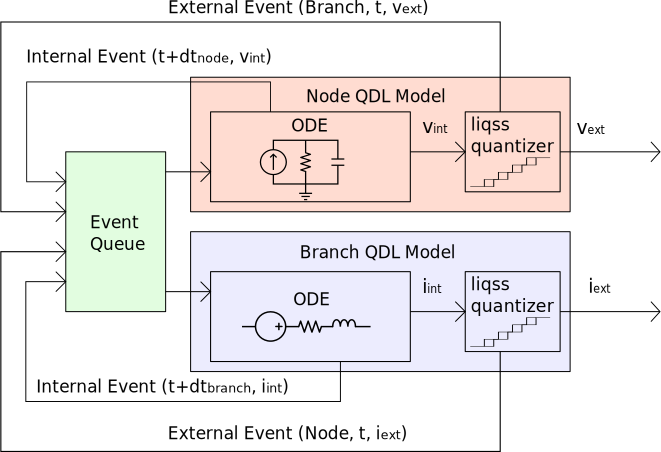
\includegraphics[width=0.6\textwidth]{qdl_sys.png}
    \caption{$2^{nd}$ order QDL system.}
    \label{fig:qdl_sys}
\end{figure}

\begin{figure}[htb]
    \centering
    \includegraphics[width=0.8\textwidth]{qdl_sys_plot.png}
    \caption{$2^{nd}$ order QDL system simulation results (where $v_{dev}$ and $i_{dev}$ are the QDL results, and $v_{ss}$ and $i_{ss}$ are the state-space reference solution results).}
    \label{fig:qdl_sys_plot}
\end{figure}

\section{Distributed Transmission Line}

The next test is a RLCG distributed transmission line model with 5 nodes and 4 branches. The first node includes the external source injection. The results for all of the node voltages ($n1$ through $n5$) and branch currents ($b1$ through $b4$) are shown in figures \ref{fig:qdl_test_9th_voltages} and \ref{fig:qdl_test_9th_currents}. A step change in the source occurs midway through the simulation to provide an additional transient disturbance.

Because the benchmark state space solution and the frequency of updates is an important metric when analyzing the results, the plots contain several types of overlaid information to help visualize these data. First, the reference implicit state space solution results are shown (dashed cyan line). The QDL results are shown as black markers, where each marker is plotted at the time of the atom's external quantized state update. Lastly, the frequency of QDL updates (how often the state is recomputed and an update event is broadcast from the atom) is shown as a histogram of updates per the span of time shown in the plot legend. Note the change in update frequency between the transient and steady-state portions of the simulation.

\begin{figure}[ht]   
    \centering     
    \includegraphics[width=0.95\linewidth]{qdl_test_9th_voltages.png}
    \caption{$9^{th}$ Order Distributed Transmission Line Voltages}     
    \label{fig:qdl_test_9th_voltages}
\end{figure} 


\begin{figure}[ht]   
    \centering     
    \includegraphics[width=0.95\linewidth]{qdl_test_9th_currents.png}
    \caption{$9^{th}$ Order Distributed Transmission Line Currents} 
    \label{fig:qdl_test_9th_currents}
\end{figure} 

\section{Very Stiff Grid Simulation}

In order to test the capabilities of the QDL method with stiff systems, a dense grid was created with a very wide range of time constants. This grid has 16 LIM nodes and 24 LIM branches (see figure \ref{fig:qdl_grid_4x4}). Each quadrant of the grid contains different levels of latency, controlled by setting the capacitance values for the nodes within in the quadrants. The eigenvalues of the system range approximately from $10^{-3}$ seconds to $10^6$ seconds, creating a stiffness ratio of approximately $10^9$. The voltages at the corner nodes are used as representative states for analysis of the results of the simulation, and are conveniently named Node 1, Node 2, Node 3, and Node 4, corresponding to their latency quadrant. 

\begin{figure}[htb]
    \centering
    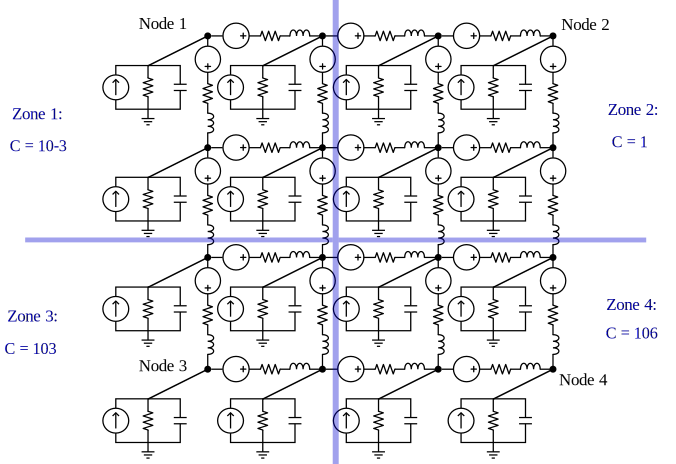
\includegraphics[width=0.9\textwidth]{qdl_grid_4x4.pdf}
    \caption{Stiff LIM grid with four latency zones.}
    \label{fig:qdl_grid_4x4}
\end{figure}   

The simulation was run for $10^4$ simulation seconds. The current injection at Node 1 is stepped from $0$ to $1 A$ at $t=0$, and from $1 A$ to $10 A$ at $t=tsim/2$ to provide a perturbation to create a dynamic response. The results are shown in figure \ref{fig:qdl_stiff_all}. Because the results from a simulation with such a large stiffness ratio are difficult to visualize on one time scale, zoomed plots of the faster transients are included for corner Node 1, Node 2 and Node 3 (see figure \ref{fig:qdl_stiff_zoom_only}). Note that the dynamic response of Node 4 is too slow to warrant a zoomed plot. 

Included in each plot are two axes, a left axis for the voltage quantity, and a right axis for the update frequency. The update frequency is the rate at which the asynchronous state updates occur in the simulation for each atom. As expected and desired, the update frequencies are relatively high during the transients, and very low or non-existent during the steady-state portions. Each plot's legend shows the update frequency histogram bin size in seconds. Note that these bin sizes vary with each plot as they were chosen for readability.  

\begin{figure}[htb]
    \centering
    \includegraphics[width=0.9\textwidth]{qdl_stiff_all.png}
    \caption{Stiff grid corner node voltage dynamic response.}
    \label{fig:qdl_stiff_all}
\end{figure}  

\begin{figure}[htb]
    \centering
    \includegraphics[width=0.9\textwidth]{qdl_stiff_zoom_only.png}
    \caption{Stiff grid corner node voltage dynamic response (zoom to transient).}
    \label{fig:qdl_stiff_zoom_only}
\end{figure} 

An implicit state space solution as a benchmark was impractical to create for this example because of the extreme stiffness and long simulation time of this simulation. The run-time of such a simulation would take many hours or days to simulate on typical desktop hardware using an implicit state space solution with a time step small enough to capture the fast dynamics. For example, a time step of $\lambda_{min}/10$ would require the solution of a 40-state system for $10^8$ time steps. The QDL system, however, requires total updates on the order of $10^5$ for all states combined, and runs in less than 5 mins on a laptop computer as a single-threaded application. Note that this is not an exhaustive performance or accuracy analysis. The quantification of computational efficiency and error will need to be part of future work. Also, because an implicit state space solution is impractical to perform on these types of the extremely stiff systems, a reasonable method of bench-marking the performance and results will have to be determined that does not require running the full simulation.

\section{DC Motor with a PWM Source}

A simulation was performed using QDL for a dc motor excited with a pulse-width modulated voltage source. This system highlights additional features of the QDL method that are not apparent in the previous transmission line or grid models. The DC motor model includes an energy-conversion coupling between the electrical and mechanical sub-networks of the system. This coupling method is very important for the simulation of power systems for the energy transfer in machines, transformers, converters, and loads. The first motor simulation, with results in figure \ref{fig:motor_1} involved a simple dc voltage source armature excitation at startup and shows the resulting armature current and rotor speed. There is an increase in mechanical torque load at the halfway mark. The system is somewhat stiff, with stiffness ratio around 10 between the electric branch and mechanical node (shaft). As expected, very few updates occur in the slower rotor speed state versus the electrical current state, and both atoms update very seldom during the steady-state portions of the simulation. 

\begin{figure}[ht]
    \label{fig:motor_1}
    \centering
    \includegraphics[width=1.0\linewidth]{motor_1.png}
    \caption{DC Motor Simulation}
\end{figure}  

To further test the QDL implementation, the DC motor model was simulated with an ideal PWM source at the armature terminals. Results for the PWM source simulation are shown for small $\Delta Q$ (figure \ref{fig:motor1_pwm_ripple}) as well as large $\Delta Q$ (figure \ref{fig:motor1_pwm_noripple}). In the first case with small $\Delta Q$, there are many updates of the external PWM state (as expected), and also many updates of the external branch current state. The current ripple is recorded in full detail, with updates on the order of 2000 per simulation second. The updates on the rotor speed node are very few and practically non-existent during steady-state. The large $\Delta Q$ simulation demonstrates the ability of QDL to ignore details like PWM-induced ripple while still effectively simulating the system. The $\Delta Q$ is chosen to be larger than the ripple magnitude, which results in the lack of ripple in the output, but more importantly very few updates in the external atom states (total updates are on the order of 10 for each atom).

\begin{figure}[ht]
    \label{fig:motor1_pwm_ripple}
    \centering
    \includegraphics[width=1.0\linewidth]{motor1_pwm_ripple2.png}
    \caption{DC Motor with PWM Source (Small quantum, with ripple)}
\end{figure}  

\begin{figure}[ht]
    \label{fig:motor1_pwm_noripple}
    \centering
    \includegraphics[width=1.0\linewidth]{motor1_pwm_noripple2.png}
    \caption{DC Motor with PWM Source (Large quantum, no ripple)}
\end{figure}  